\documentclass[../../main.tex]{subfiles}

\begin{document}
\graphicspath{{img/}{06_result/img/}}

\chapter{Kết quả và kết luận}

\section{Kết quả}
Hình \ref{fig:cuda_implement_result} là kết quả mô phỏng của CUDA-GMapping. Ta thấy chương trình đã có thể giải quyết bài toán SLAM trong môi trường mô phỏng mà cụ thể ở đây là turtle-world trong Gazebo.
\begin{figure}[H]
    \begin{center}
        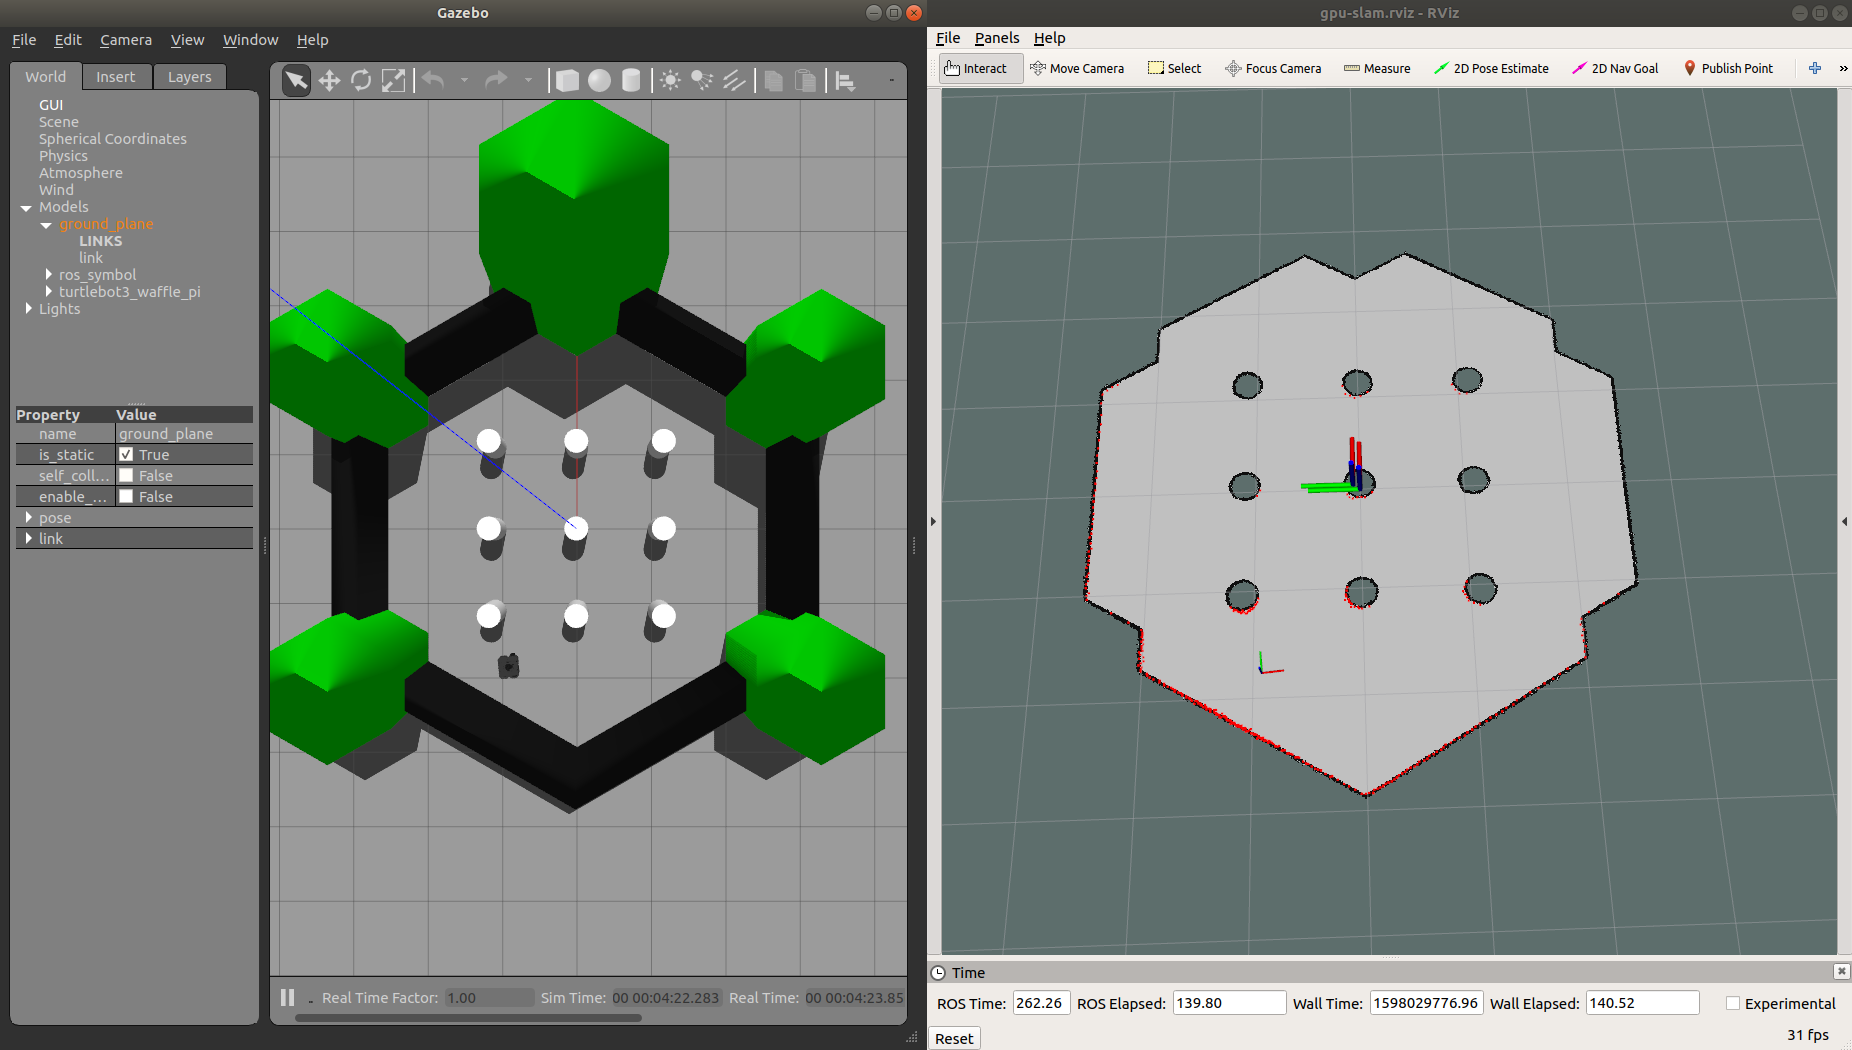
\includegraphics[scale=0.25]{turtle_world.png}
    \end{center}
    \caption{Kết quả sau khi implement GMapping bằng CUDA}
    \label{fig:cuda_implement_result}
\end{figure}

Hình \ref{fig:gpu_vs_cpu} so sánh tốc độ chạy trong mỗi vòng lặp của CUDA implementation và CPU implementation với thời gian chạy của CPU đã được chia 10.

Kết quả mô phỏng hình \ref{fig:gpu_vs_cpu} được thực hiện trên máy tính có CPU core i7-8700K và GPU GTX-1060 6GB.

Vì CPU implementation của GMmaping có thời gian chạy cho mỗi vòng lặp tăng lên sau một số vòng lặp nhất định nên kết quả trên đồ thị lấy giá trị trung bình thời gian chạy cho 50 vòng lặp đầu tiên.

Từ đồ thị có thể thấy GPU cải thiện tốc độ chạy cho thuật toán một cách đáng kể, nhất là khi số lượng particle tăng lên cao.
\begin{figure}[H]
    \begin{center}
        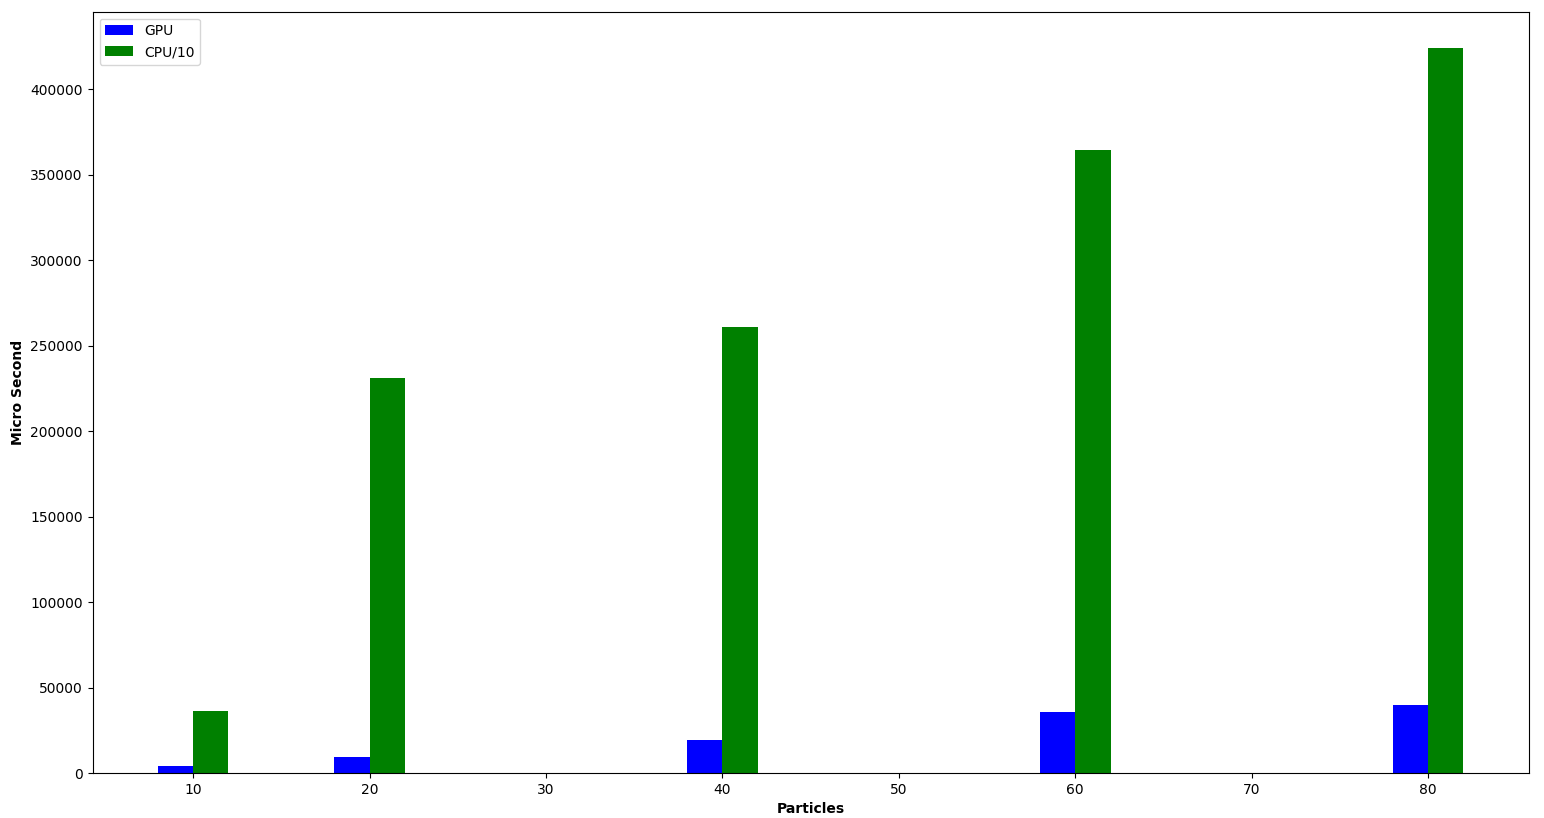
\includegraphics[scale=0.3]{gpu_vs_cpu.png}
    \end{center}
    \caption{GPU và CPU}
    \label{fig:gpu_vs_cpu}
\end{figure}

\section{Kết luận}
GMapping CUDA implementation có các ưu điểm và nhược điểm sau:

Ưu điểm:
\begin{itemize}
    \item CUDA implementation giảm thời gian chaỵ của mỗi vòng lặp một cách đáng kể.
\end{itemize}

Nhược điểm:
\begin{itemize}
    \item Đầu tư phần cứng có GPU hỗ trợ CUDA
    \item Số lượng RAM của GPU có hạn hơn so với của CPU. Do đó, số lượng particle tối đa của GPU-implementation sẽ hạn chế hơn so với CPU-implementation nếu kích thước môi trường lớn hoặc độ phân giải của map cao.
\end{itemize}
\end{document}